% Created 2017-03-29 Wed 08:47
% Intended LaTeX compiler: pdflatex
\documentclass[presentation]{beamer}
\usepackage[utf8]{inputenc}
\usepackage[T1]{fontenc}
\usepackage{graphicx}
\usepackage{grffile}
\usepackage{longtable}
\usepackage{wrapfig}
\usepackage{rotating}
\usepackage[normalem]{ulem}
\usepackage{amsmath}
\usepackage{textcomp}
\usepackage{amssymb}
\usepackage{capt-of}
\usepackage{hyperref}
\usetheme{default}
\author{Logan Woodbury}
\date{\textit{[2017-03-21 Tue]}}
\title{Alternation Turing Machines}
\hypersetup{
 pdfauthor={Logan Woodbury},
 pdftitle={Alternation Turing Machines},
 pdfkeywords={},
 pdfsubject={A presentation on Alternating Turing Machines},
 pdfcreator={Emacs 24.5.1 (Org mode 9.0.5)}, 
 pdflang={English}}
\begin{document}

\maketitle
\begin{frame}{Outline}
\tableofcontents
\end{frame}

\begin{block}{Outline}
\begin{block}{Nondeterministic Turing Machines}
\end{block}
\begin{block}{Alternation}
\end{block}
\begin{block}{ATIME and ASPACE}
\end{block}
\begin{block}{\(\Sigma_{\text{i}}\)-alternating Turing Machines and \(\Pi_{\text{i}}\)-alternating Turing Machines}
\end{block}
\end{block}

\begin{frame}[label={sec:org950a81c}]{Nondeterministic Turing Machines}
\begin{block}{Basic Idea}
\begin{block}{Deterministic Finite Automata \(\rightarrow\) Nondeterministic Finite Automata}
\end{block}
\end{block}
\begin{block}{Basic Idea}
\begin{block}{Deterministic Finite Automata \(\rightarrow\) Nondeterministic Finite Automata}
\end{block}
\begin{block}{Turing Machine \(\rightarrow\) ?}
\end{block}
\end{block}
\begin{block}{Basic Idea}
\begin{block}{Deterministic Finite Automata \(\rightarrow\) Nondeterministic Finite Automata}
\end{block}
\begin{block}{Turing Machine \(\rightarrow\) Nondeterministic Turing Machine}
\end{block}
\end{block}
\begin{block}{Basic Idea}
\begin{block}{Deterministic Finite Automata \(\rightarrow\) Nondeterministic Finite Automata}
\end{block}
\begin{block}{Turing Machine \(\rightarrow\) Nondeterministic Turing Machine}
\end{block}
\begin{block}{P \(\rightarrow\) NP}
\end{block}
\end{block}
\begin{block}{Formal Description}
\begin{block}{\(M = (Q,\Sigma,\iota,\_,A,\delta)\)}
\begin{block}{\(Q\) is the set of states}
\end{block}
\begin{block}{\(\Sigma\) is the Tape Alphabet}
\end{block}
\begin{block}{\(\iota\) is the initial state: \(\iota \in Q\)}
\end{block}
\begin{block}{\(\_\) is the blank symbol: \(\_ \in \Sigma\)}
\end{block}
\begin{block}{\(A\) is the set of accept states: \(A \in Q\)}
\end{block}
\begin{block}{\(\delta\) is the transition function: \(\delta \subset (Q \backslash A x \Sigma) \rightarrow P(Q x \Sigma x \{L,R\})\)}
\end{block}
\end{block}
\end{block}

\begin{block}{Example: SAT}
\begin{block}{Assign all possible assignments of variables concurrently}
\end{block}
\begin{block}{Check if any of them evaluate to true\ldots{} concurrently!}
\end{block}
\begin{block}{If you find one that does, accept!}
\end{block}
\end{block}
\end{frame}
\begin{frame}[label={sec:orgf916c10}]{Alternation}
\begin{block}{Basic Idea}
\begin{block}{NTMs are kinda\ldots{} easy to please?}
\end{block}
\end{block}
\begin{block}{Basic Idea}
\begin{block}{NTMs are kinda\ldots{} easy to please?}
\end{block}
\begin{block}{All states are logical "or's"}
\end{block}
\end{block}
\begin{block}{Basic Idea}
\begin{block}{How about we have a system where we could have alternating or's and and's?}
\end{block}
\end{block}
\begin{block}{Basic Idea}
\begin{center}
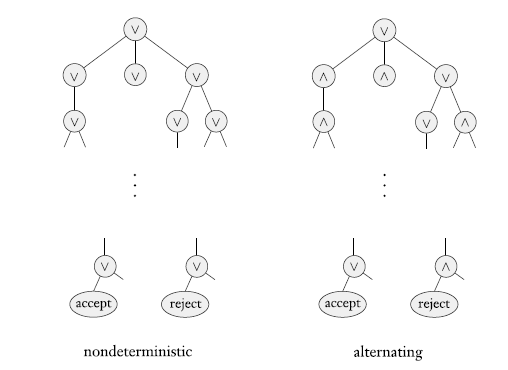
\includegraphics[width=.9\linewidth]{./atm_tree.png}
\end{center}
\end{block}
\begin{block}{Basic Idea}
\begin{block}{Turing Machines \(\rightarrow\) Nondeterministic Turing Machines \(\rightarrow\) Alternating Turing Machines}
\end{block}
\begin{block}{P \(\rightarrow\) NP \(\rightarrow\) AP}
\end{block}
\end{block}
\begin{block}{Formal Description}
\begin{block}{\(M = (Q,\Gamma,\delta,q_{0},g)\)}
\begin{block}{\(Q\) is the still set of states}
\end{block}
\begin{block}{\(\Gamma\) is now the Tape Alphabet}
\end{block}
\begin{block}{\(\delta\) is still the transition function: \(\delta : (Q x \Sigma) \rightarrow P(Q x \Gamma x \{L,R\})\)}
\end{block}
\begin{block}{\(q_{0}\) is now the initial state: \(q_{0} \in Q\)}
\end{block}
\begin{block}{\(g\) is a function that specifies the \emph{type} of each state \(g : Q \rightarrow \{\land,\lor,accept,reject\}\)}
\end{block}
\end{block}
\end{block}
\begin{block}{Examples: TAUT (Tautology)}
\begin{block}{\(TAUT = \{\langle \Phi \rangle | \Phi\) is a tautology\(\}\)}
\begin{block}{Universally select all possible assignments to the variables of \(\Phi\) (\(\land\))}
\end{block}
\begin{block}{Evaluate these assignments to see if they are true}
\end{block}
\begin{block}{If all the assignments accept, accept! Otherwise\ldots{} reject!}
\end{block}
\end{block}
\end{block}

\begin{block}{Examples: SEXY}
\begin{block}{L = $\backslash${S | S is a series of 1's in a positive multiple of 3, followed by an even amount of 0's, or the inverse (3x 0's followed by 2y 1's)$\backslash$}}
\end{block}
\begin{block}{Spent a lot of time on this one!}
\end{block}
\begin{block}{Not exactly a particularly difficult problem to solve anyhow, but\ldots{}}
\end{block}
\end{block}

\begin{block}{Examples: MIN-FORMULA}
\begin{block}{\(MIN-FORMULA = \{\langle \Phi \rangle | \Phi\) is the smallest possible way to express that formula\(\}\)}
\begin{block}{\emph{Universally} select all formulas \(\psi\) that are shorter than \(\Phi\) (\(\land\))}
\end{block}
\begin{block}{\emph{Existentially} select an assignment to the variables of \(\Phi\) (\(\lor\))}
\end{block}
\begin{block}{Evaluate both \(\Phi\) and \(\psi\), accept if they have the same values, otherwise reject!}
\end{block}
\end{block}
\end{block}
\end{frame}

\begin{frame}[label={sec:org6ea825d}]{ATIME and ASPACE}
\begin{block}{TIME and (Relative Dimension In) SPACE}
\begin{center}
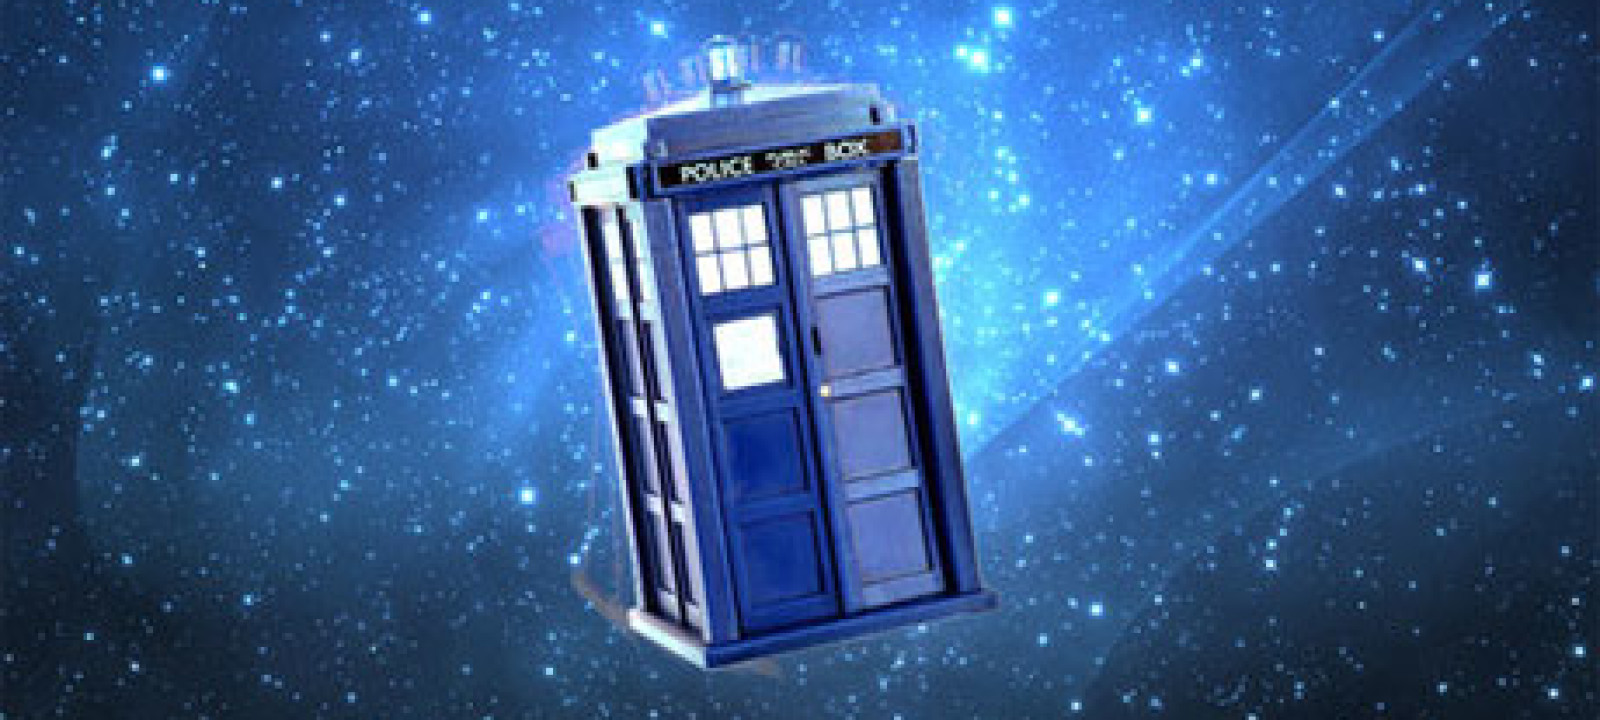
\includegraphics[width=.9\linewidth]{./tardis.jpg}
\end{center}
\end{block}
\begin{block}{ATIME and ASPACE (ATARDIAS?)}
\begin{block}{\(ATIME(t(n)) = \{L|L\) is decided by an \(O(t(n))\) time alternating Turing Machine \(\}\)}
\end{block}
\begin{block}{\(ASPACE(f(n)) = \{L|L\) is decided by an \(O(f(n))\) space alternating Turing Machine \(\}\)}
\end{block}
\end{block}
\begin{block}{Relations!}
\begin{block}{For \(f(n) \ge n\), we have \(ATIME(f(n)) \subseteq SPACE(f(n)) \subseteq ATIME(f^{2}(n))\)}
\end{block}
\begin{block}{For \(f(n) \ge \log n\), we have \(ASPACE(f(n)) = TIME(2^{O(f(n))})\)}
\end{block}
\end{block}
\end{frame}
\begin{frame}[label={sec:orgfcecea4}]{\(\Sigma_{\text{i}}\)-alternating Turing Machines and \(\Pi_{\text{i}}\)-alternating Turing Machines}
\begin{block}{Definitions}
\begin{block}{\$\(\Sigma_{\text{i}}\)\$-alternating Turing machine is an alternating Turing machine that on the longest possible branch has \(i runs\) universal or existential steps}
\end{block}
\begin{block}{\$\(\Sigma_{\text{i}}\)\$-alternating Turing machines start with existential steps}
\end{block}
\begin{block}{\$\(\Pi_{\text{i}}\)\$-alternating Turing machines start with universal steps}
\end{block}
\end{block}
\begin{block}{\(\Sigma_{\text{i}}\)TIME, \(\Pi_{\text{i}}\)TIME, \(\Sigma_{\text{i}}\)SPACE, \(\Pi_{\text{i}}\)SPACE}
\begin{block}{\ldots{}Not hard to figure out what all these are}
\end{block}
\end{block}
\begin{block}{\(\Sigma_{i}P\) and \(\Pi _{i}P\)}
\begin{block}{\(\Sigma_{i}P = \cup_{k \in \Re} \Sigma_{i}TIME(n^{k})\)}
\end{block}
\begin{block}{\(\Pi_{i}P = \cup_{k \in \Re} \Pi_{i}TIME(n^{k})\)}
\end{block}
\end{block}
\begin{block}{\(\Sigma_{i}P\) and \(\Pi _{i}P\)}
\begin{block}{\(\Sigma_{i}P = \cup_{k \in \Re} \Sigma_{i}TIME(n^{k})\)}
\end{block}
\begin{block}{\(\Pi_{i}P = \cup_{k \in \Re} \Pi_{i}TIME(n^{k})\)}
\end{block}
\begin{block}{\(\Sigma_{1}P\)}
\end{block}
\end{block}
\begin{block}{\(\Sigma_{i}P\) and \(\Pi _{i}P\)}
\begin{block}{\(\Sigma_{i}P = \cup_{k \in \Re} \Sigma_{i}TIME(n^{k})\)}
\end{block}
\begin{block}{\(\Pi_{i}P = \cup_{k \in \Re} \Pi_{i}TIME(n^{k})\)}
\end{block}
\begin{block}{\(NP = \Sigma_{1}P\)}
\end{block}
\end{block}
\begin{block}{\(\Sigma_{i}P\) and \(\Pi _{i}P\)}
\begin{block}{\(\Sigma_{i}P = \cup_{k \in \Re} \Sigma_{i}TIME(n^{k})\)}
\end{block}
\begin{block}{\(\Pi_{i}P = \cup_{k \in \Re} \Pi_{i}TIME(n^{k})\)}
\end{block}
\begin{block}{\(NP = \Sigma_{1}P\)}
\end{block}
\begin{block}{\(coNP = \Pi_{1}P\)}
\end{block}
\end{block}
\begin{block}{\(\Sigma_{i}P\) and \(\Pi _{i}P\)}
\begin{block}{\(\Sigma_{i}P = \cup_{k \in \Re} \Sigma_{i}TIME(n^{k})\)}
\end{block}
\begin{block}{\(\Pi_{i}P = \cup_{k \in \Re} \Pi_{i}TIME(n^{k})\)}
\end{block}
\begin{block}{\(NP = \Sigma_{1}P\)}
\end{block}
\begin{block}{\(coNP = \Pi_{1}P\)}
\end{block}
\begin{block}{\(MIN-FORMULA \in \Pi_{2}P\)}
\end{block}
\end{block}
\begin{block}{\(\Sigma_{i}P\) and \(\Pi _{i}P\)}
\begin{block}{\(\Sigma_{i}P = \cup_{k \in \Re} \Sigma_{i}TIME(n^{k})\)}
\end{block}
\begin{block}{\(\Pi_{i}P = \cup_{k \in \Re} \Pi_{i}TIME(n^{k})\)}
\end{block}
\begin{block}{\(NP = \Sigma_{1}P\)}
\end{block}
\begin{block}{\(coNP = \Pi_{1}P\)}
\end{block}
\begin{block}{\(MIN-FORMULA \in \Pi_{2}P\)}
\end{block}
\begin{block}{\(SEXY \in \Sigma_{3}P\)}
\end{block}
\end{block}
\begin{block}{\(\Sigma_{i}P\) and \(\Pi _{i}P\)}
\begin{block}{\(\Sigma_{i}P = \cup_{k \in \Re} \Sigma_{i}TIME(n^{k})\)}
\end{block}
\begin{block}{\(\Pi_{i}P = \cup_{k \in \Re} \Pi_{i}TIME(n^{k})\)}
\end{block}
\begin{block}{\(NP = \Sigma_{1}P\)}
\end{block}
\begin{block}{\(coNP = \Pi_{1}P\)}
\end{block}
\begin{block}{\(MIN-FORMULA \in \Pi_{2}P\)}
\end{block}
\begin{block}{\(SEXY \in \Sigma_{3}P\)}
\end{block}
\begin{block}{(It is also most definitely in P)}
\end{block}
\end{block}
\end{frame}
\begin{frame}[label={sec:org6a9fcd6}]{Conclusion}
\end{frame}
\end{document}
